\documentclass[11pt]{article}
\usepackage{theme}
\usepackage{shortcuts}

\usepackage{graphicx}
\usepackage{amsmath,amssymb}
\usepackage{booktabs}
\usepackage[numbers]{natbib}
\usepackage{float}

\usepackage{algorithm}
\usepackage{algorithmicx}
\usepackage{algpseudocode}

\usepackage{tikz}
\usetikzlibrary{positioning, arrows.meta}

% Document parameters
% Document title
\title{Interactions - MVA 2025/2026
      \\ \Large{Project Assignment}
      \\ \Large{Mean-Field Neural Networks with Graphon Heterogeneity \\ for Systemic Risk Control}}

\author{
Adonis JAMAL \email{adonis.jamal@student-cs.fr}\\
Fotios KAPOTOS \email{fotiskapotos@gmail.com}
}

\date{April 2026}

%%%%%%%%%%%%%%%%%%%%%%%
% ABSTRACT
%%%%%%%%%%%%%%%%%%%%%%%


% ==============================================================================
% ================================== DOCUMENT ==================================  
% ==============================================================================
\begin{document}
\maketitle

% ==============================================================================
% SECTION : INTRODUCTION AND CONTRIBUTIONS
% ==============================================================================
\section{Introduction and Contributions}

\citet{pham2024mfnn} introduce mean-field neural networks (MFNNs) to solve McKean-Vlasov (MKV) control problems: as the population size $N \to \infty$, propagation of chaos \citep{sznitman1991propagation} yields a single controlled MKV SDE whose optimal policy maps a probability measure to a control action, requiring architectures that operate on $\PPP_2(\RR)$, the Wasserstein space of probability measures with finite second moment. The paper proposes bin-density and cylindrical encoders and eight training algorithms, validated on the linear-quadratic systemic risk benchmark of \citet{carmona2015systemic} against an exact Riccati solution.

This project aims to address what happens when a policy learned under the mean-field hypothesis is deployed on a finite, structurally heterogeneous network. The MF limit assumes an infinite exchangeable population on a complete interaction graph; real financial systems violate both. Once these assumptions are relaxed, cascading defaults emerge as a collective phenomenon whose statistics are invisible in the smooth MF cost functional. This places the project at the intersection of interacting particle systems, agent-based models, and extreme-event theory: the finite discrete system exhibits a phase transition in the inter-bank coupling $q$, with power-law cascade-size distributions near the critical point $q^*$. Network heterogeneity is modelled via a graphon \citep{lovasz2012large}, replacing the complete graph with core-periphery or Erdős-Rényi structures.

Our contributions are: (i) a faithful implementation of Algorithms 1 (global DP) and 6 (global BSDE) with both encoders, validated against the Riccati benchmark on all six initial distributions; (ii) an empirical characterisation of the MF-limit breakdown as $N$ grows from 10 to 1000 across three topologies; (iii) a phase-transition analysis quantifying the policy-induced shift $\Delta q^* > 0$ in the critical coupling; and (iv) an out-of-distribution robustness evaluation of the frozen policy on unseen initial laws and heterogeneous graphs.

% ==============================================================================
% SECTION : PAPER OVERVIEW
% ==============================================================================
\section{Paper Overview}

\citet{pham2024mfnn} address the numerical solution of McKean-Vlasov control (MKV) problems, which arise as the cooperative mean-field limit of $N$-agent stochastic systems. The controlled state evolves as
\begin{equation}\label{eq:mkv-sde-main}
  \dd X_t = b(X_t, \PP_{X_t}, \alpha_t)\,\dd t + \sigma(X_t, \PP_{X_t})\,\dd W_t, \qquad X_0 \sim \mu_0,
\end{equation}
and the social planner minimises
\begin{equation}\label{eq:mkv-cost-main}
  v(\mu_0) = \inf_\alpha \EE\!\left[\int_0^T f(X_t, \PP_{X_t}, \alpha_t)\,\dd t + g(X_T, \PP_{X_T})\right].
\end{equation}
The fundamental difficulty is representational: both $v$ and the optimal feedback $\alpha^*(t, x, \mu)$ are defined on $\PPP_2(\RR^d)$, making standard finite-dimensional networks inapplicable. From the perspective of the Interactions course, \eqref{eq:mkv-sde-main} is precisely the continuum limit of an IPS: under propagation of chaos \citep{sznitman1991propagation}, the $N$-particle system decouples as $N \to \infty$, with each agent governed by a nonlinear SDE whose coefficients depend self-consistently on the law of its own solution.

\textbf{Mean-field neural network architectures.} The paper introduces two architectures that lift standard feedforward networks to measure-valued inputs. The \emph{bin-density encoder} discretises $\mu$ on a fixed grid $\mathcal{K}$ into $K$ bins, producing a normalised histogram $p^\mu \in \RR^K$; the policy network is $\Phi_\theta(t, x, p^\mu)$. The \emph{cylindrical encoder} computes a learnable moment embedding
\begin{equation}\label{eq:cylindrical-main}
  z = \frac{1}{N}\sum_{n=1}^N \varphi_\theta(X^{(n)}) \in \RR^q
\end{equation}
via an inner network $\varphi_\theta$, passed to an outer network $\Psi_\theta(t, x, z)$. Both are permutation-invariant and satisfy a universal approximation theorem on $\PPP_2(\RR^d)$.

\textbf{Training algorithms.} The paper proposes eight algorithms in two families. Algorithm 1 (global Dynamic Programming) minimises $\hat{J}(\theta)$ end-to-end by differentiating through the Euler simulation of \eqref{eq:mkv-sde-main}. Algorithms 4-8 exploit the FBSDE characterisation derived from the Pontryagin maximum principle: setting $Y_t = V(t, X_t, \PP_{X_t})$ (the value function along the optimal trajectory) and $Z_t = \sigma^\top \partial_x V(t, X_t, \PP_{X_t})$, the backward equation reads
\begin{equation}\label{eq:bsde-main}
  \dd Y_t = -f(X_t, \PP_{X_t}, \alpha^*_t)\,\dd t + Z_t\,\dd W_t, \qquad Y_T = g(X_T, \PP_{X_T}),
\end{equation}
and the control is recovered via the adjoint $P_t = \mathcal{U}(t, X_t, \PP_{X_t}) = \partial_x V + \EE_{\xi \sim \PP_{X_t}}[\partial_\mu V(\cdot)(X_t)]$ as $\alpha^* = \hat{a}(X_t, \PP_{X_t}, P_t)$. Algorithm 6 (global BSDE) learns $(Y, Z)$ jointly over all time steps by minimising the terminal residual $\EE[\|Y_T - g(X_T, \PP_{X_T})\|^2]$.

We focus on Algorithms 1 and 6 because they are the canonical representatives of their respective families at global scope: both train a single network over all time steps simultaneously, avoiding the compounding errors of the sequential (local) variants. Algorithm 1 is the simplest baseline and stress-tests the DP approach; Algorithm 6 provides the BSDE alternative grounded in the Pontryagin principle. The paper itself reports that these two are the most accurate algorithms on the 1D systemic risk benchmark, and their structural symmetry (same training scope, different optimality characterisation) makes the comparison informative.

\textbf{Systemic risk benchmark.} Validation uses the LQ systemic risk model of \citet{carmona2015systemic}: the log-monetary reserve of a representative bank satisfies
\begin{equation}\label{eq:systemic-main}
  \dd X_t = \bigl(\kappa(\EE[X_t] - X_t) + \alpha_t\bigr)\,\dd t + \sigma\,\dd W_t,
\end{equation}
with cost $\tilde{f}(x,\bar x, a) = \tfrac{1}{2}a^2 - qa(\bar x - x) + \tfrac{\eta}{2}(\bar x - x)^2$ and terminal cost $\tilde{g}(x,\bar x) = \tfrac{c}{2}(x - \bar x)^2$. This model is chosen to be relevant on three counts: (i) it is an IPS with all-to-all coupling whose MF limit is \eqref{eq:systemic-main}; (ii) the finite-$N$ system produces cascading defaults, an emergent phenomenon invisible in the smooth MF cost; and (iii) the LQ structure admits an exact Riccati solution $v(t,\mu) = Q_t \int(x-\bar\mu)^2\,\mu(\dd x) + \sigma^2\int_t^T Q_s\,\dd s$, providing ground-truth for validation.



% ==============================================================================
% SECTION : METHODOLOGY
% ==============================================================================
\section{Methodology}



% ==============================================================================
% SECTION : DATA AND EXPERIMENTAL SETUP
% ==============================================================================
\section{Data and Experimental Setup}



% ==============================================================================
% SECTION : RESULTS
% ==============================================================================
\section{Results}



% ==============================================================================
% SECTION : CONCLUSION AND DISCUSSION
% ==============================================================================
\section{Conclusion and Discussion}



% ==============================================================================
% SECTION : BIBLIOGRAPHY
% ==============================================================================
\bibliographystyle{plainnat}
\bibliography{bibliography}



% ==============================================================================
% SECTION : APPENDIX
% ==============================================================================
\newpage
\appendix

% ------------------------------------------------------------------------------
% APPENDIX A : McKean-Vlasov Control
% ------------------------------------------------------------------------------
\begin{figure}[htbp]
\centering
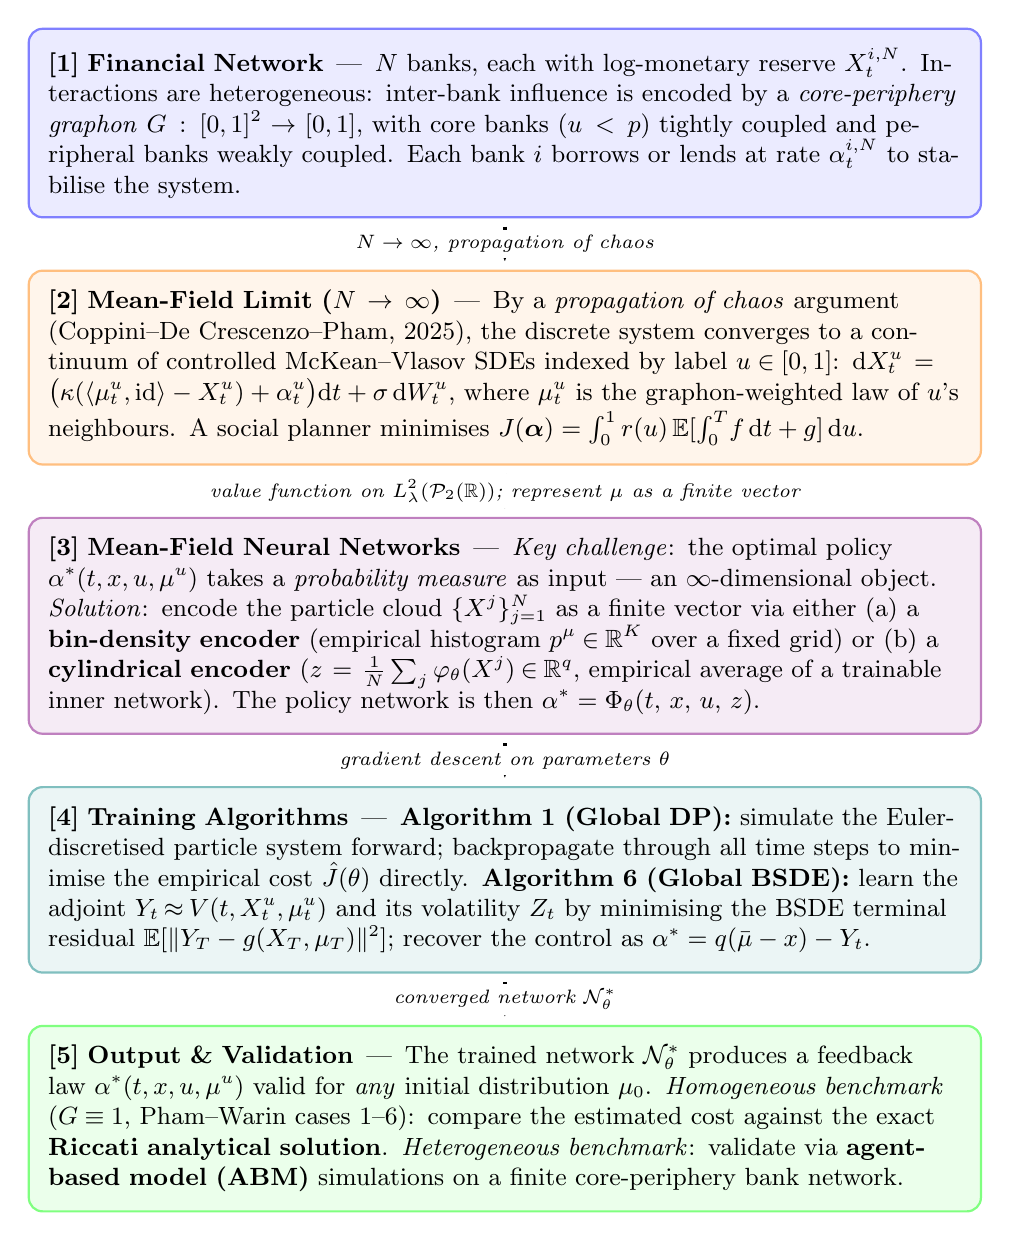
\begin{tikzpicture}[
  font=\small,
  box/.style={
    rectangle, rounded corners=5pt,
    minimum width=12cm, text width=11.6cm,
    draw, line width=0.8pt,
    inner sep=7pt, align=left
  },
  arr/.style={-Stealth, line width=1.2pt, shorten >=3pt, shorten <=3pt},
  steplabel/.style={midway, fill=white, inner sep=2pt, font=\scriptsize\itshape}
]

\node[box, fill=blue!8, draw=blue!50] (s1) {
  \textbf{[1]\;Financial Network}\enspace---\enspace
  $N$ banks, each with log-monetary reserve $X^{i,N}_t$.
  Interactions are heterogeneous: inter-bank influence is encoded by a
  \emph{core-periphery graphon} $G:[0,1]^2\!\to\![0,1]$, with core banks ($u<p$)
  tightly coupled and peripheral banks weakly coupled.
  Each bank $i$ borrows or lends at rate $\alpha^{i,N}_t$ to stabilise the system.
};

\node[box, fill=orange!8, draw=orange!50, below=0.65cm of s1] (s2) {
  \textbf{[2]\;Mean-Field Limit ($N\!\to\!\infty$)}\enspace---\enspace
  By a \emph{propagation of chaos} argument (Coppini--De Crescenzo--Pham, 2025), the
  discrete system converges to a continuum of controlled McKean--Vlasov SDEs indexed
  by label $u\!\in\![0,1]$:
  $\mathrm{d}X^u_t = \bigl(\kappa(\langle\mu^u_t,\mathrm{id}\rangle-X^u_t)+\alpha^u_t\bigr)\mathrm{d}t
  +\sigma\,\mathrm{d}W^u_t$,
  where $\mu^u_t$ is the graphon-weighted law of $u$'s neighbours.
  A social planner minimises
  $J(\boldsymbol\alpha) = \int_0^1 r(u)\,\mathbb{E}[\int_0^T\! f\,\mathrm{d}t + g]\,\mathrm{d}u$.
};

\node[box, fill=violet!8, draw=violet!50, below=0.65cm of s2] (s3) {
  \textbf{[3]\;Mean-Field Neural Networks}\enspace---\enspace
  \emph{Key challenge}: the optimal policy $\alpha^*(t,x,u,\mu^u)$ takes a
  \emph{probability measure} as input --- an $\infty$-dimensional object.
  \emph{Solution}: encode the particle cloud $\{X^{j}\}_{j=1}^N$ as a finite vector
  via either (a)~a \textbf{bin-density encoder}
  (empirical histogram $p^\mu\!\in\!\mathbb{R}^K$ over a fixed grid)
  or (b)~a \textbf{cylindrical encoder}
  ($z = \tfrac{1}{N}\sum_j\varphi_\theta(X^j)\!\in\!\mathbb{R}^q$,
  empirical average of a trainable inner network).
  The policy network is then $\alpha^* = \Phi_\theta(t,\,x,\,u,\,z)$.
};

\node[box, fill=teal!8, draw=teal!50, below=0.65cm of s3] (s4) {
  \textbf{[4]\;Training Algorithms}\enspace---\enspace
  \textbf{Algorithm~1 (Global DP):} simulate the Euler-discretised particle system
  forward; backpropagate through all time steps to minimise the empirical cost
  $\hat J(\theta)$ directly.
  \textbf{Algorithm~6 (Global BSDE):} learn the adjoint
  $Y_t\!\approx\!V(t,X^u_t,\mu^u_t)$ and its volatility $Z_t$ by minimising the
  BSDE terminal residual
  $\mathbb{E}[\lVert Y_T - g(X_T,\mu_T)\rVert^2]$;
  recover the control as $\alpha^* = q(\bar\mu - x) - Y_t$.
};

\node[box, fill=green!8, draw=green!50, below=0.65cm of s4] (s5) {
  \textbf{[5]\;Output \& Validation}\enspace---\enspace
  The trained network $\mathcal{N}_\theta^*$ produces a feedback law
  $\alpha^*(t,x,u,\mu^u)$ valid for \emph{any} initial distribution $\mu_0$.
  \emph{Homogeneous benchmark} ($G\!\equiv\!1$, Pham--Warin cases~1--6):
  compare the estimated cost against the exact \textbf{Riccati analytical solution}.
  \emph{Heterogeneous benchmark}: validate via \textbf{agent-based model (ABM)}
  simulations on a finite core-periphery bank network.
};

\draw[arr] (s1.south) -- node[steplabel] {$N\to\infty$, propagation of chaos} (s2.north);
\draw[arr] (s2.south) -- node[steplabel] {value function on $L^2_\lambda(\mathcal{P}_2(\mathbb{R}))$; represent $\mu$ as a finite vector} (s3.north);
\draw[arr] (s3.south) -- node[steplabel] {gradient descent on parameters $\theta$} (s4.north);
\draw[arr] (s4.south) -- node[steplabel] {converged network $\mathcal{N}_\theta^*$} (s5.north);

\end{tikzpicture}
\caption{%
  End-to-end project pipeline.
  \textbf{Blue}~[1]: agent-based financial system with graphon-structured heterogeneous interactions.
  \textbf{Orange}~[2]: McKean--Vlasov mean-field formulation obtained as the $N\to\infty$ limit.
  \textbf{Purple}~[3]: mean-field neural network architectures that map a probability measure
  (infinite-dimensional input) to a finite-dimensional representation.
  \textbf{Teal}~[4]: two training strategies --- dynamic programming (Algorithm~1) and
  backward SDE (Algorithm~6) --- from \citet{pham2024mfnn}.
  \textbf{Green}~[5]: output feedback policy and validation against exact analytical
  and agent-based simulation benchmarks.
}
\label{fig:pipeline}
\end{figure}


\section{McKean--Vlasov Control Problem}\label{sec:appendix-mkv}

We recall the general framework for mean-field control (MFC), also called McKean--Vlasov (MKV) control, following the formulation of \citet{pham2024mfnn}.

\subsection{Controlled McKean--Vlasov SDE}

Let $(\Omega, \mathcal{F}, \mathbb{F} = (\mathcal{F}_t)_{t \ge 0}, \PP)$ be a filtered probability space supporting a $d$-dimensional Brownian motion $W$. The controlled state process $X = (X_t)_{0 \le t \le T}$, valued in $\RR^d$, is governed by the mean-field stochastic differential equation:
\begin{equation}\label{eq:mkv-sde}
  \dd X_t = b(X_t, \PP_{X_t}, \alpha_t)\,\dd t + \sigma(X_t, \PP_{X_t}, \alpha_t)\,\dd W_t, \qquad 0 \le t \le T, \quad X_0 \sim \mu_0,
\end{equation}
where $\mu_0 \in \PPP_2(\RR^d)$ is the initial distribution, $\alpha = (\alpha_t)_t$ is a progressively measurable control process valued in $A \subset \RR^m$, and $\PP_{X_t}$ denotes the law of $X_t$ under $\PP$. The coefficients $b : \RR^d \times \PPP_2(\RR^d) \times A \to \RR^d$ and $\sigma : \RR^d \times \PPP_2(\RR^d) \times A \to \RR^{d \times d}$ satisfy standard Lipschitz regularity assumptions.

Here $\PPP_2(\RR^d)$ denotes the Wasserstein space of probability measures with finite second moment, equipped with the 2-Wasserstein distance:
\begin{equation}\label{eq:wasserstein}
  \mathcal{W}_2(\mu, \nu) = \left( \inf_{X \sim \mu, Y \sim \nu} \EE\left[ d(X, Y)^2 \right] \right)^{1/2},
\end{equation}
where $X, Y$ are random with law given respectively by $\mu$ and $\nu$.

\begin{remark}
  The key feature of \eqref{eq:mkv-sde} compared to a standard controlled SDE is that the coefficients depend on the \emph{law} $\PP_{X_t}$ of the state, making the system intrinsically infinite-dimensional. This reflects the mean-field interaction in a large population of cooperative agents governed by a social planner.
\end{remark}

\subsection{Cost Functional and Value Function}

The social planner seeks to minimize the cost functional:
\begin{equation}\label{eq:mkv-cost}
  J(\alpha) = \EE\left[\int_0^T f(X_t, \PP_{X_t}, \alpha_t)\,\dd t + g(X_T, \PP_{X_T})\right],
\end{equation}
where $f : \RR^d \times \PPP_2(\RR^d) \times A \to \RR$ is the running cost and $g : \RR^d \times \PPP_2(\RR^d) \to \RR$ is the terminal cost. The value function is:
\begin{equation}\label{eq:value-fn}
  v(\mu_0) = \inf_{\alpha \in \mathcal{A}} J(\alpha).
\end{equation}

A crucial observation is that $v$ is defined on the \emph{Wasserstein space} $\PPP_2(\RR^d)$, making it a function on an infinite-dimensional space. This is the central computational challenge: standard neural networks, which take finite-dimensional inputs, cannot directly represent mappings on $\PPP_2(\RR^d)$.

\subsection{Dynamic Programming Characterization}

The decoupled value function $V : [0,T] \times \RR^d \times \PPP_2(\RR^d) \to \RR$ satisfies the backward recursion:
\begin{equation}\label{eq:dp-recursion}
  V(t, X_t, \PP_{X_t}) = \inf_{\alpha \in \mathcal{A}} \EE\left[\int_t^{t+h} f(X_s, \PP_{X_s}, \alpha_s)\,\dd s + V(t+h, X_{t+h}, \PP_{X_{t+h}}) \;\middle|\; \mathcal{F}_t\right],
\end{equation}
with terminal condition $V(T, x, \mu) = g(x, \mu)$, and $v(\mu_0) = \EE[V(0, X_0, \mu_0)]$.

Sending $h \to 0$ yields the \emph{Master Bellman equation} on $[0,T) \times \RR^d \times \PPP_2(\RR^d)$, which involves the Lions derivative $\partial_\mu V$ on the Wasserstein space \citep{carmona2018mfg1}. The optimal feedback control takes the form:
\begin{equation}\label{eq:optimal-control}
  \alpha^\star(t, x, \mu) = \hat{a}\big(x, \mu, \mathcal{U}(t,x,\mu), \partial_x \mathcal{U}(t,x,\mu)\big),
\end{equation}
where $\mathcal{U}(t,x,\mu) = \partial_x V(t,x,\mu) + \EE_{\xi \sim \mu}[\partial_\mu V(t,\xi,\mu)(x)]$, and $\hat{a}$ minimizes the Hamiltonian:
\begin{equation}
  H(x,\mu,p,M,a) := b(x,\mu,a) \cdot p + \tfrac{1}{2} \sigma\sigma^\top(x,\mu,a) \cdot M + f(x,\mu,a).
\end{equation}

\subsection{Forward-Backward SDE Characterization (Pontryagin)}

When $\sigma(x,\mu)$ does not depend on the control, setting $Y_t = V(t, X_t, \PP_{X_t})$ and $Z_t = \sigma(X_t, \PP_{X_t})^\top \partial_x V(t, X_t, \PP_{X_t})$, one obtains the forward-backward SDE system:
\begin{equation}\label{eq:fbsde}
  \begin{cases}
    \dd X_t = b\big(X_t, \PP_{X_t}, \hat{a}(X_t, \PP_{X_t}, P_t)\big)\,\dd t + \sigma(X_t, \PP_{X_t})\,\dd W_t, & X_0 \sim \mu_0, \\[4pt]
    \dd Y_t = -f\big(X_t, \PP_{X_t}, \hat{a}(X_t, \PP_{X_t}, P_t)\big)\,\dd t + Z_t \cdot \dd W_t, & Y_T = g(X_T, \PP_{X_T}),
  \end{cases}
\end{equation}
for $0 \leq t \leq T$, where $P_t = \mathcal{U}(t, X_t, \PP_{X_t})$. This characterization forms the basis of the backward SDE-based algorithms (Algorithms 4-8 in \citet{pham2024mfnn}).


% ------------------------------------------------------------------------------
% APPENDIX B : Mean-Field Neural Networks
% ------------------------------------------------------------------------------
\section{Mean-Field Neural Network Architectures}\label{sec:appendix-mfnn}

Since the value function and optimal control are mappings on the Wasserstein space, one requires neural network architectures capable of taking a probability measure as input. \citet{pham2024mfnn} introduce two such architectures.

\subsection{Bin Density Network}

The \emph{bin density} network represents $\mu \in \PPP_2(\RR^d)$ by discretizing its density on a fixed rectangular domain $\mathcal{K} \subset \RR^d$ divided into $K$ equal-volume bins $\{\mathrm{Bin}(k)\}_{k=1}^K$ with centers $x_k$ and bin volume $h = \lambda^d(\mathcal{K})/K$. The network takes the form:
\begin{equation}\label{eq:bin-density}
  \mathcal{N}(\mu)(x) = \Phi\big(x, \, p^\mu\big), \qquad p^\mu_k = \frac{p_\mu(x_k)}{\sum_{j=1}^K p_\mu(x_j)\,h}, \quad k = 1, \ldots, K,
\end{equation}
where $p_\mu$ is the density of $\mu$ and $\Phi : \RR^d \times \RR^K \to \RR^p$ is a standard feedforward neural network. The bin weight vector $p^\mu \in \RR^K$ provides a finite-dimensional representation of the measure.

\begin{remark}
  The bin density network requires a bounded support $\mathcal{K}$, whose choice affects accuracy. An iterative procedure is proposed in \citet{pham2024mfnn} to adaptively select $\mathcal{K}$. The method is primarily effective for $d = 1$ due to the curse of dimensionality in binning.
\end{remark}

\subsection{Cylindrical Network}

The \emph{cylindrical} network is defined as:
\begin{equation}\label{eq:cylindrical}
  \mathcal{N}(\mu)(\cdot) = \Psi\big(\cdot, \, \langle \varphi, \mu \rangle\big), \qquad \langle \varphi, \mu \rangle := \int_{\RR^d} \varphi(x)\,\mu(\dd x) \in \RR^q,
\end{equation}
where $\varphi : \RR^d \to \RR^q$ is an \emph{inner} feedforward network (encoding the measure into a latent space of dimension $q$), and $\Psi : \RR^d \times \RR^q \to \RR^p$ is an \emph{outer} feedforward network. Given samples $X^{(n)} \sim \mu$, $n = 1, \ldots, N$, the cylindrical function is approximated by:
\begin{equation}
  \mathcal{N}(\mu)(\cdot) \approx \Psi\left(\cdot, \; \frac{1}{N}\sum_{n=1}^N \varphi(X^{(n)})\right).
\end{equation}

Both architectures satisfy a universal approximation property on the Wasserstein space and are permutation-invariant with respect to the particle ordering.

\subsection{Algorithm Overview}

\citet{pham2024mfnn} propose eight algorithms divided into two families:
\begin{itemize}
  \item \textbf{Dynamic Programming (DP) based:} Algorithms 1-3:
    \begin{enumerate}
      \item Algorithm 1 (\emph{Global DP}): global learning of the feedback control via direct minimization of $J(\alpha)$ over all time steps simultaneously.
      \item Algorithm 2 (\emph{Policy iteration}): alternates between policy evaluation and policy improvement at each time step.
      \item Algorithm 3 (\emph{Value iteration}): sequentially learns the control and the value function backward in time.
    \end{enumerate}
  \item \textbf{Backward SDE / Pontryagin based:} Algorithms 4-8: exploit the FBSDE characterization \eqref{eq:fbsde} with various global or local loss functions.
\end{itemize}

For this project, we primarily target \textbf{Algorithm 1} (global DP) and \textbf{Algorithm 6} (global BSDE), as they offer the best trade-off between implementation simplicity and accuracy on the systemic risk benchmark.


% ------------------------------------------------------------------------------
% APPENDIX C : Systemic Risk Model
% ------------------------------------------------------------------------------
\section{Systemic Risk Model}\label{sec:appendix-systemic}

We consider the mean-field model of systemic risk introduced by \citet{carmona2015systemic} in the context of mean-field games, adapted here to the cooperative (MFC) setting as in Section~5.1.1 of \citet{pham2024mfnn}.

\subsection{Model Formulation}

The log-monetary reserve of a representative bank evolves according to the mean-reverting controlled McKean--Vlasov dynamics:
\begin{equation}\label{eq:systemic-sde}
  \dd X_t = \big(\kappa(\EE[X_t] - X_t) + \alpha_t\big)\,\dd t + \sigma\,\dd W_t, \qquad X_0 \sim \mu_0,
\end{equation}
where $\kappa > 0$ is the mean-reversion rate reflecting inter-bank lending, $\sigma > 0$ is the volatility, and $\alpha_t$ is the rate of borrowing/lending to a central bank (the control).

The parameter $\kappa$ governs the strength of interaction: each bank's log-reserve is pulled toward the population mean $\EE[X_t]$. In the $N$-bank finite system, this corresponds to a fully connected (complete graph) interaction where each bank $i$ is influenced by $\bar{X}_t^N = \frac{1}{N}\sum_{j=1}^N X_t^{j,N}$.

\subsection{Cost Functional}

The central bank (social planner) minimizes:
\begin{equation}\label{eq:systemic-cost}
  J(\alpha) = \EE\left[\int_0^T \tilde{f}(X_t, \EE[X_t], \alpha_t)\,\dd t + \tilde{g}(X_T, \EE[X_T])\right] \to v(\mu_0) = \inf_\alpha J(\alpha),
\end{equation}
with running and terminal costs:
\begin{equation}\label{eq:systemic-costs-detail}
  \tilde{f}(x, \bar{x}, a) = \frac{1}{2}a^2 - qa(\bar{x} - x) + \frac{\eta}{2}(\bar{x} - x)^2, \qquad \tilde{g}(x, \bar{x}) = \frac{c}{2}(x - \bar{x})^2,
\end{equation}
where $q, \eta, c > 0$ with $q^2 \le \eta$. The term $\frac{1}{2}a^2$ penalizes the control effort, the term $-qa(\bar{x} - x)$ incentivizes banks far from the mean to borrow/lend more, and the terminal cost penalizes dispersion around the mean at maturity. The convexity of the objective function with respect to the control process ensures the convergence of the global algorithm in the linear-quadratic example.

\subsection{Analytical Solution}

This linear-quadratic (LQ) problem admits an analytical solution via a Riccati equation \citep{carmona2018mfg1}:
\begin{equation}\label{eq:systemic-value}
  v(t, \mu) = \int_{\RR} V(t, x, \mu)\,\mu(\dd x) = Q_t \int_{\RR} (x - \bar{\mu})^2\,\mu(\dd x) + \sigma^2 \int_t^T Q_s\,\dd s,
\end{equation}
where $\bar{\mu} = \int x\,\mu(\dd x)$ and $Q_t$ solves a Riccati ODE involving $\kappa, q, \eta, c$. The analytical value serves as a ground-truth benchmark for validating the neural network algorithms.

\subsection{Benchmark Parameters}

Following \citet{pham2024mfnn}, the standard test parameters are $\sigma = 1$, $\kappa = 0.6$, $q = 0.8$, $T = 0.2$, $c = 2$, $\eta = 2$. In the current implementation, the six benchmark initial laws are matched exactly as follows, with $Y, \bar Y \sim \mathcal{N}(0,1)$ independent, $P \sim \mathrm{Bernoulli}(1/2)$, and $U \sim \mathrm{Unif}(0,1)$:
\begin{align*}
  \text{Case 1: } X_0 &= 0.2Y, \\
  \text{Case 2: } X_0 &= 0.3 + 0.05Y, \\
  \text{Case 3: } X_0 &= 0.05Y, \\
  \text{Case 4: } X_0 &= P(-k + \theta Y) + (1-P)(k + \theta \bar Y), \quad k = \frac{\sqrt{3}}{10}, \; \theta = 0.1, \\
  \text{Case 5: } X_0 &= P(-k + \theta Y) + (1-P)(-k + \theta \bar Y), \quad k = 0.25, \; \theta = 0.1, \\
  \text{Case 6: } X_0 &= \big(-\mathbf{1}_{\{\lfloor 3U \rfloor = 0\}}k + \mathbf{1}_{\{\lfloor 3U \rfloor = 1\}}k\big) + \theta Y, \quad k = 0.3, \; \theta = 0.07.
\end{align*}
For these laws, the analytical values computed from the Riccati formula are approximately $0.4849$ for Cases 1 and 4, $0.3625$ for Cases 2 and 3, $0.3870$ for Case 5, and $0.5662$ for Case 6. The equalities $v(0,\mu_0^{(1)}) = v(0,\mu_0^{(4)})$ and $v(0,\mu_0^{(2)}) = v(0,\mu_0^{(3)})$ follow from the fact that the LQ value depends only on the initial variance.

\begin{remark}[Cascade interpretation]
  When the interaction parameter $\kappa$ is large relative to the volatility, the mean-reverting force creates strong coupling. In the uncontrolled discrete system ($\alpha \equiv 0$), if a subset of banks crosses a default threshold $\theta$ (i.e., $X_t^i < \theta$), the resulting drop in $\bar{X}_t^N$ pulls all remaining banks downward, potentially triggering a \emph{cascade} or \emph{avalanche} of defaults. This systemic risk mechanism is what the control aims to mitigate.
\end{remark}

\subsection{Exact Implementation Choices and Preliminary Sweep}

The current repository now exposes the two Pham--Warin algorithms targeted in this project using the same modeling choices as in the benchmark setup. Algorithm 1 is implemented as a global control-learning method: a time-dependent mean-field neural network $\mathcal{N}_\theta(t,\mu)(x)$ is trained by simulating the Euler scheme for the particle system and minimizing the empirical counterpart of the full objective $J(\alpha)$. Algorithm 6 is implemented as a global MKV BSDE method for the systemic-risk adjoint system, learning an initial adjoint map $\mathcal{U}_\theta(\mu)(x)$ together with a time-dependent process network $\mathcal{Z}_\theta(t,\mu)(x)$, and recovering the induced control through
\[
  \alpha_t^\star \approx q(\EE[X_t] - X_t) - P_t.
\]
On the architecture side, the cylindrical encoder uses the empirical average of an inner feature map, while the bin encoder now uses hard histogram counts on a fixed support interval rather than a smoothed Gaussian proxy.

To obtain a first implementation-level comparison, we ran a moderate local sweep on CPU over all six benchmark cases, both encoders, and both algorithms, with $N = 64$ particles, $N_T = 12$ time steps, batch size $8$, and $60$ optimization iterations per run. This is intentionally smaller than the paper's full training budget, so the numbers below should be read as consistency checks rather than direct reproductions of the published tables. The main qualitative outcome is that Algorithm 1 behaves similarly with the two encoders at this scale, while Algorithm 6 is more stable with the bin encoder, which is consistent with the observation reported by \citet{pham2024mfnn} on difficult one-dimensional benchmarks.

\begin{table}[H]
  \centering
  \begin{tabular}{lcc}
    \toprule
    Method and encoder & Average final training loss & Average induced policy cost \\
    \midrule
    Algorithm 1 + bins & 0.1622 & -- \\
    Algorithm 1 + cylindrical & 0.1617 & -- \\
    Algorithm 6 + bins & 0.0127 & 0.1606 \\
    Algorithm 6 + cylindrical & 0.0276 & 0.1644 \\
    \bottomrule
  \end{tabular}
  \caption{Moderate local benchmark sweep for the current implementation across Cases 1-6. The induced policy cost is reported only for Algorithm 6, where the learned adjoint induces the feedback control.}
  \label{tab:systemic-preliminary-sweep}
\end{table}

These runs indicate that the repository now matches the paper at the level of benchmark laws, encoder choice, and algorithmic interface, while a higher-budget experiment remains necessary to compare quantitatively against the published Pham--Warin tables.


% ------------------------------------------------------------------------------
% APPENDIX D : Graphon Particle Systems
% ------------------------------------------------------------------------------
\section{Nonlinear Graphon Mean-Field Systems}\label{sec:appendix-graphon}

We summarize the framework of \citet{coppini2025graphon}, which extends classical mean-field limits to heterogeneous particle systems on graphs.

\subsection{Graphons}

A \emph{graphon} is a measurable symmetric function $G : [0,1]^2 \to [0,1]$. It arises as the limit of sequences of dense graphs in the cut-distance topology \citep{lovasz2012large}. Given an $N$-vertex graph with adjacency matrix $(a_{ij})$, the associated step-function graphon is:
\begin{equation}
  G_N(u,v) = a_{\lceil Nu \rceil, \lceil Nv \rceil}, \qquad (u,v) \in [0,1]^2.
\end{equation}
The graphon encodes heterogeneous interaction weights: $G(u,v)$ measures the strength of interaction between agents with labels $u$ and $v$.

\subsection{Nonlinear Graphon Particle System}

Consider a system of $N$ interacting particles where particle $i$ has label $u_i = i/N \in [0,1]$. Its state $X^{i,N}$ evolves as:
\begin{equation}\label{eq:graphon-particle}
  \dd X_t^{i,N} = b\!\left(X_t^{i,N}, \, \hat{\mu}_t^{i,N}\right)\dd t + \sigma\!\left(X_t^{i,N}, \, \hat{\mu}_t^{i,N}\right)\dd W_t^i, \qquad 0 \leq t \leq T, \qquad i = 1, \ldots, N,
\end{equation}
where $\hat{\mu}_t^{i,N}$ is the \emph{local empirical measure} of particle $i$:
\begin{equation}\label{eq:local-empirical}
  \hat{\mu}_t^{i,N} = \frac{\sum_{j=1}^N G(u_i, u_j)\,\delta_{X_t^{j,N}}}{\sum_{j=1}^N G(u_i, u_j)}.
\end{equation}
The key feature is that the interaction of particle $i$ with the population is weighted by the graphon $G$: strongly connected agents (high $G(u_i, u_j)$) contribute more to the local measure than weakly connected ones.

\begin{remark}
  When $G \equiv 1$, the local empirical measure reduces to the standard empirical measure $\hat{\mu}_t^N = \frac{1}{N}\sum_{j=1}^N \delta_{X_t^{j,N}}$, recovering the classical homogeneous mean-field setting.
\end{remark}

The drift and diffusion coefficients $b, \sigma : \RR^d \times \PPP_2(\RR^d) \to \RR^d$ (resp.\ $\RR^{d \times d}$) satisfy Lipschitz regularity:
\begin{assumption}\label{ass:lipschitz}
  There exists $K > 0$ such that $|b(x,\mu) - b(x',\mu')| + |\sigma(x,\mu) - \sigma(x',\mu')| \le K(|x-x'| + \mathcal{W}_2(\mu,\mu'))$ for all $x, x' \in \RR^d$ and $\mu, \mu' \in \PPP_2(\RR^d)$.
\end{assumption}

\subsection{Fubini Extension and Limit System}\label{sec:fubini}

When $N \to \infty$, the limit system consists of an \emph{uncountable} family of processes $(X_t^u)_{u \in [0,1]}$ indexed by the label $u$. To rigorously define this infinite collection, \citet{coppini2025graphon} use a \emph{Fubini extension} of the standard probability space.

\begin{definition}[Fubini extension, {\citet[Definition~3.1]{coppini2025graphon}}]
  An extension $([0,1] \times \Omega, \, \mathcal{I} \otimes \mathcal{F}, \, \lambda \otimes \PP)$ of the product space is a \emph{Fubini extension} if for every $\mathcal{I} \otimes \mathcal{F}$-measurable process $f : [0,1] \times \Omega \to \RR$ that is integrable:
  \begin{enumerate}
    \item $u \mapsto f(u, \omega)$ is $\mathcal{I}$-measurable for $\PP$-a.e.\ $\omega$,
    \item $\omega \mapsto f(u, \omega)$ is $\mathcal{F}$-measurable for $\lambda$-a.e.\ $u$,
    \item The Fubini theorem holds: $\int_{[0,1] \times \Omega} f\,\dd(\lambda \otimes \PP) = \int_{[0,1]} \left(\int_\Omega f(u,\omega)\,\dd\PP(\omega)\right)\dd\lambda(u)$.
  \end{enumerate}
\end{definition}

The limit system on this extended space reads: for $\lambda$-a.e.\ $u \in [0,1]$,
\begin{equation}\label{eq:graphon-limit}
  \dd X_t^u = b\!\left(X_t^u, \, \mu_t^u\right)\dd t + \sigma\!\left(X_t^u, \, \mu_t^u\right)\dd W_t^u, \qquad X_0^u \sim \mu_0^u,
\end{equation}
where $\mu_t^u \in \PPP_2(\RR^d)$ is the \emph{graphon-weighted law}:
\begin{equation}\label{eq:graphon-law}
  \mu_t^u = \frac{\int_0^1 G(u,v)\,\PP_{X_t^v}\,\dd v}{\int_0^1 G(u,v)\,\dd v},
\end{equation}
and $(W^u)_{u \in [0,1]}$ is a family of independent Brownian motions on the Fubini extension.

\subsection{Main Convergence Results}

\begin{theorem}[Law of Large Numbers, {\citet[Theorem~4.1]{coppini2025graphon}}]\label{thm:lln}
  Under Assumption~\ref{ass:lipschitz} and standard regularity on $G$ and the initial conditions, the local empirical measures converge:
  \begin{equation}
    \lim_{N \to \infty} \frac{1}{N} \sum_{i=1}^N \EE\left[ \sup_{0 \leq t \leq T} \left| X_t^{i, N} - X_t^{u_i} \right| \right] = \lim_{N \to \infty} \frac{1}{N} \sum_{i=1}^N \EE\left[ \int_{0}^{t} \mathcal{W}_2^2 ([G_N \delta_s^N]^{u_i}, [G\mu_s]^{u_i}) ds \right] = 0,
  \end{equation}
  where $\mu_t^u$ is the graphon-weighted law from the limit system \eqref{eq:graphon-limit}.
\end{theorem}

\begin{theorem}[Propagation of Chaos, {\citet[Theorem~4.2]{coppini2025graphon}}]\label{thm:poc}
  Under the same assumptions, for any finite collection of labels $u_1, \ldots, u_k \in [0,1]$, the joint law of $(X^{u_1,N}, \ldots, X^{u_k,N})$ converges to the product law $\PP_{X^{u_1}} \otimes \cdots \otimes \PP_{X^{u_k}}$ as $N \to \infty$. In other words, particles with distinct labels become asymptotically independent, each governed by the nonlinear process \eqref{eq:graphon-limit}.
\end{theorem}

The convergence rate depends on the dimension $d$ and matches the Fournier--Guillin rate \citep{fournier2015rate} for the convergence of empirical measures in Wasserstein distance.


% ------------------------------------------------------------------------------
% APPENDIX E : MFC of Non-Exchangeable Systems
% ------------------------------------------------------------------------------
\section{Mean-Field Control of Non-Exchangeable Systems}\label{sec:appendix-nonexch}

We summarize the theoretical contribution of \citet{decrescenzo2026mfc}, which establishes the dynamic programming principle for MFC problems with graphon-structured heterogeneous interactions.

\subsection{Controlled Graphon Particle System}

The controlled dynamics of particle $i \in \{1, \ldots, N\}$ in the graphon system with heterogeneous coefficients is:
\begin{equation}\label{eq:nonexch-particle}
  \dd X_t^{i,N} = b\!\left(u_i, X_t^{i,N}, \alpha_t^{i,N}, \frac{1}{N_i}\sum_{j=1}^N G(u_i, u_j)\,\delta_{X_t^{j,N}}\right)\dd t + \sigma\!\left(u_i, X_t^{i,N}, \alpha_t^{i,N}, \frac{1}{N_i}\sum_{j=1}^N G(u_i, u_j)\,\delta_{X_t^{j,N}}\right)\dd W_t^{u_i},
\end{equation}
where $u_i = i/N$ is the label, $N_i = \sum_{j=1}^N G(u_i, u_j)$ is the degree, and $\alpha^{i,N}$ is the control for agent $i$. Note that the coefficients $b$ and $\sigma$ now explicitly depend on the label $u_i$, allowing for agent heterogeneity beyond the graphon interaction structure.

\subsection{Mean-Field Limit and Cost Functional}

In the $N \to \infty$ limit, the social planner minimizes the cost functional over the continuum of agents:
\begin{equation}\label{eq:nonexch-cost}
  J(\boldsymbol{\alpha}) = \int_0^1 r(u)\,\EE\left[\int_0^T f\!\left(u, X_t^u, \alpha_t^u, \mu_t^u\right)\dd t + g\!\left(u, X_T^u, \mu_T^u\right)\right]\dd u,
\end{equation}
where $r : [0,1] \to \RR_+$ is a label-weighting function, and the state and graphon-weighted law $(\mu_t^u)_{u,t}$ are defined as in \eqref{eq:graphon-limit}--\eqref{eq:graphon-law}. The collection of marginal laws $\boldsymbol{\mu}_t = (\mu_t^u)_{u \in [0,1]}$ lives in the space $L^2_\lambda(\PPP_2(\RR^d))$, the set of $L^2$-functions from $[0,1]$ into the Wasserstein space.

\subsection{Law Invariance and Value Function}

A key result of \citet{decrescenzo2026mfc} is the \emph{law invariance property}: the value function depends on the state of the system only through the collection of marginal laws $\boldsymbol{\mu} = (\PP_{X^u})_{u \in [0,1]}$. This allows defining:
\begin{equation}\label{eq:nonexch-value}
  v(t, \boldsymbol{\mu}) = \inf_{\boldsymbol{\alpha}} J_{t,\boldsymbol{\mu}}(\boldsymbol{\alpha}),
\end{equation}
where $\boldsymbol{\mu} \in L^2_\lambda(\PPP_2(\RR^d))$ is the initial collection of laws at time $t$.

\subsection{Dynamic Programming Principle}

\begin{theorem}[DPP, {\citet[Theorem~4.1]{decrescenzo2026mfc}}]
  Under standard regularity assumptions, the value function $v$ satisfies the dynamic programming principle: for all $0 \le t \le s \le T$ and $\boldsymbol{\mu} \in L^2_\lambda(\PPP_2(\RR^d))$,
  \begin{equation}
    v(t, \boldsymbol{\mu}) = \inf_{\boldsymbol{\alpha}} \left\{ \int_0^1 r(u)\,\EE\left[\int_t^s f\!\left(u, X_r^u, \alpha_r^u, \mu_r^u\right)\dd r\right]\dd u + v(s, \boldsymbol{\mu}_s) \right\}.
  \end{equation}
\end{theorem}

Moreover, \citet{decrescenzo2026mfc} derive a chain rule for smooth functions along flows of marginal laws, and prove that $v$ is a viscosity solution to a Bellman equation on $L^2_\lambda(\PPP_2(\RR^d))$.

\begin{remark}[Open problem]
  While \citet{decrescenzo2026mfc} establish the theoretical DPP and Bellman equation for graphon MFC, \emph{no numerical algorithm} has been proposed to solve these problems computationally. This project aims to bridge this gap by extending the mean-field neural network algorithms of \citet{pham2024mfnn} to the graphon-heterogeneous setting.
\end{remark}


% ------------------------------------------------------------------------------
% APPENDIX F : Project Formulation
% ------------------------------------------------------------------------------
\section{Project Formulation: Heterogeneous Systemic Risk}\label{sec:appendix-formulation}

We now combine the elements from the preceding sections to formulate the specific model studied in this project.

\subsection{Heterogeneous Systemic Risk SDE}

We extend the systemic risk model of Section~\ref{sec:appendix-systemic} by introducing agent labels $u \in [0,1]$ and a graphon interaction structure. The log-monetary reserve of agent $u$ evolves as:
\begin{equation}\label{eq:hetero-sde}
  \dd X_t^u = \left(\kappa(u)\left(\langle \mu_t^u, \mathrm{id}\rangle - X_t^u\right) + \alpha_t^u\right)\dd t + \sigma(u)\,\dd W_t^u, \qquad X_0^u \sim \mu_0^u,
\end{equation}
where $\kappa(u)$ and $\sigma(u)$ are label-dependent parameters, $\mu_t^u$ is the graphon-weighted local measure \eqref{eq:graphon-law}, and $\langle \mu_t^u, \mathrm{id} \rangle = \int x\,\mu_t^u(\dd x)$ is the local weighted mean perceived by agent $u$.

\subsection{Core-Periphery Graphon}

We choose a \emph{core-periphery} block graphon as the interaction structure:
\begin{equation}\label{eq:core-periphery}
  G(u,v) = \begin{cases}
    q_{cc} & \text{if } u,v \in [0, p], \\
    q_{cp} & \text{if } u \in [0,p], v \in (p,1] \text{ or vice versa}, \\
    q_{pp} & \text{if } u,v \in (p, 1],
  \end{cases}
\end{equation}
where $p \in (0,1)$ is the fraction of core (hub) agents, and $q_{cc} > q_{cp} > q_{pp}$ reflects the stylized fact that core banks are strongly interconnected, have moderate connections to peripheral banks, and peripheral banks interact weakly with each other.

\begin{remark}
  This graphon is a step-function with three blocks. It captures the key heterogeneity of financial networks (a dense core of systemically important institutions surrounded by a sparser periphery) while remaining simple enough for systematic analysis. Hub agents ($u \in [0,p]$) have higher effective degree and therefore perceive a denser local empirical measure.
\end{remark}

\subsection{Modified Cost Functional}

The social planner minimizes:
\begin{equation}\label{eq:hetero-cost}
  J(\boldsymbol{\alpha}) = \int_0^1 r(u)\,\EE\left[\int_0^T \left(\frac{1}{2}(\alpha_t^u)^2 - q\,\alpha_t^u\big(\langle \mu_t^u, \mathrm{id}\rangle - X_t^u\big) + \frac{\eta}{2}\big(\langle \mu_t^u, \mathrm{id}\rangle - X_t^u\big)^2\right)\dd t + \frac{c}{2}\big(X_T^u - \langle \mu_T^u, \mathrm{id}\rangle\big)^2\right]\dd u,
\end{equation}
with $r(u)$ a label-weighting function (\eg $r \equiv 1$ for uniform weighting, or $r(u)$ proportional to the degree for degree-weighted social welfare).

\subsection{Modified Neural Network Input}

To learn the label-dependent optimal control $\alpha^\star(t, x, u, \mu^u)$, we modify the mean-field neural network architectures of Section~\ref{sec:appendix-mfnn} by concatenating the label $u$ to the input:
\begin{itemize}
  \item \textbf{Bin density}: $\mathcal{N}(\mu^u)(t, x, u) = \Phi(t, x, u, p^{\mu^u})$ where $p^{\mu^u}$ is the bin weight of the \emph{local} empirical measure,
  \item \textbf{Cylindrical}: $\mathcal{N}(\mu^u)(t, x, u) = \Psi\!\left(t, x, u, \frac{1}{N_i}\sum_{j=1}^N G(u, u_j)\,\varphi(X^j)\right)$.
\end{itemize}

The key insight is that the network must learn a \emph{family} of control policies indexed by the label $u$, rather than a single policy. This is computationally feasible because the label space $[0,1]$ is one-dimensional, and the network can smoothly interpolate across labels.

\subsection{Connection to Course Concepts}

This formulation connects to the core themes of the Interactions course:
\begin{itemize}
  \item \textbf{Agent-Based Models}: the discrete $N$-bank system \eqref{eq:nonexch-particle} is an ABM with heterogeneous interactions on a network.
  \item \textbf{Emergence}: cascading defaults arise as emergent phenomena from local interactions when the control is insufficient or mis-specified.
  \item \textbf{Interacting Particle Systems}: the graphon particle system \eqref{eq:graphon-particle} is an IPS whose macroscopic behavior is described by the graphon mean-field limit.
  \item \textbf{Mean-field approximation}: the gap between the finite-$N$ ABM and the infinite-population limit quantifies when the mean-field approximation breaks down, particularly under heterogeneity.
\end{itemize}


\end{document}